\section{Results and Discussion}
\label{sec:results}

\subsection{System Design Completion}

\subsubsection{Mechanical Structural Design}

The structural design follows the department requirement of presenting dimensioned
2D drawings first, followed by 3D CAD models and cross-sectional assembly views.
All 2D dimensioned orthographic drawings were produced in SolidWorks with
institution title blocks, part numbers, and material specifications. CAD models
confirm dimensional fit, threaded-rod routing, and component sub-assembly
relationships within the 95\,mm cylindrical avionics bay envelope. The complete
set of manufacturing drawings and 3D models is presented in Appendix~\ref{app:cad}.

Figure~\ref{fig:res_cross_section} shows the labelled cross-sectional view of the
avionics bay and Figure~\ref{fig:res_parts_list} shows the full assembly parts list
with component identifications.

\begin{figure}[!htbp]
  \centering
  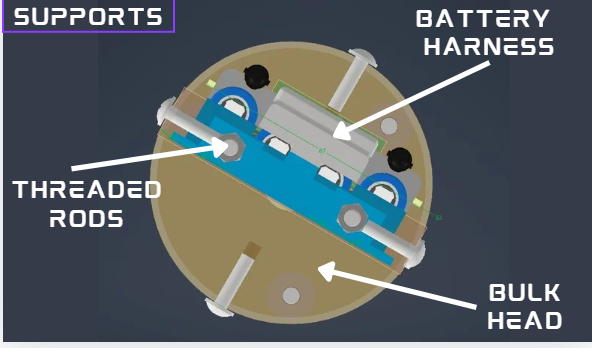
\includegraphics[width=0.90\textwidth]{images/Labeled/Assembly_Cross_section.PNG}
  \caption{Labelled cross-sectional avionics bay showing component stacking and
    structural clearances.}
  \label{fig:res_cross_section}
\end{figure}

\begin{figure}[!htbp]
  \centering
  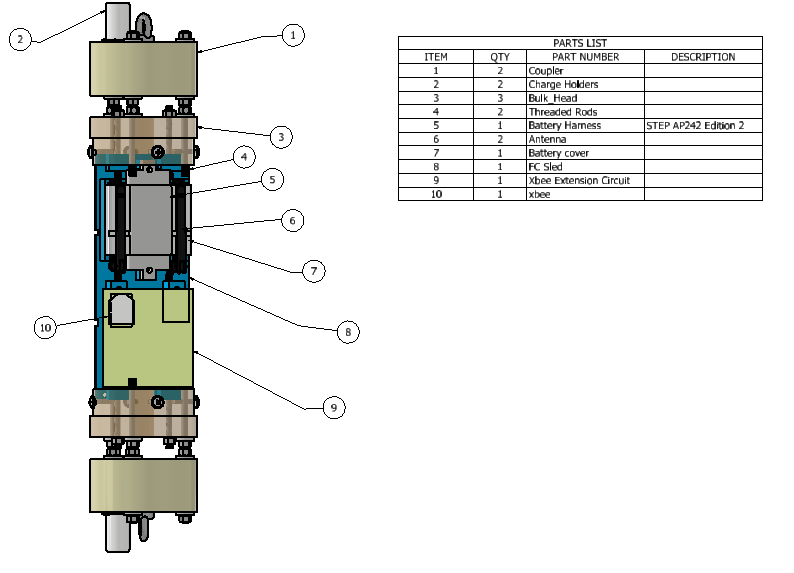
\includegraphics[width=\textwidth]{images/Labeled/Full_assemly_Parts_List.PNG}
  \caption{Full avionics bay assembly parts list with component identification
    and mounting assignments.}
  \label{fig:res_parts_list}
\end{figure}

\begin{figure}[!htbp]
  \centering
  
\includegraphics[width=0.75\textwidth]{{images/mechanical/Full Integration in avionics bay.jpeg}}
  \caption{Full avionics bay integration within the cylindrical fiberglass
    airframe section.}
  \label{fig:res_full_integration}
\end{figure}

\subsubsection{3D Printing Process}

The PETG avionics sled, battery holders, and ejection cap components were sliced
in Prusa Slicer at 0.20\,mm layer height, 40\% infill, with support material
enabled everywhere. Figure~\ref{fig:sliced_model} shows the sliced build plate
ready for export, with a total estimated print time of 18\,h\,25\,min and
189.32\,g of PETG filament consumed across all parts.



\subsubsection{Electrical Circuit Design}

EasyEDA schematics for the flight computer and base station were developed from
preliminary Fritzing layouts and iterated through multiple revisions. The final
flight computer PCB layout and the base station schematic are presented in
Figures~\ref{fig:fc_pcb_layout} and \ref{fig:bs_pcb_layout}. A complete
EasyEDA view of the full flight computer PCB routing is shown in
Figure~\ref{fig:fc_xbee_easyeda}.

\begin{figure}[!htbp]
  \centering
  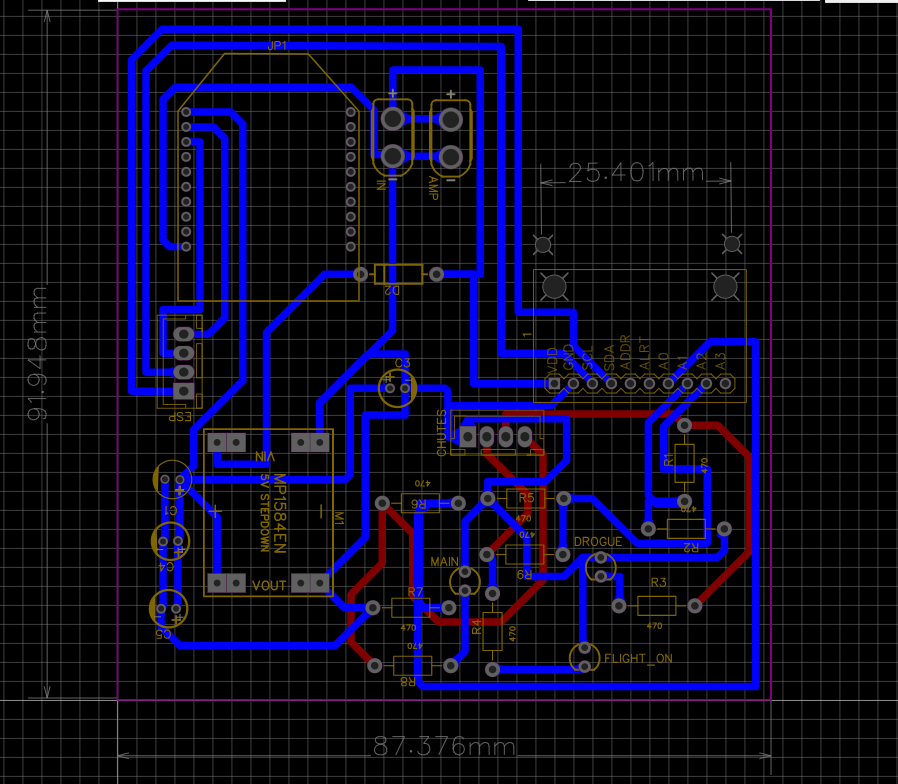
\includegraphics[width=0.85\textwidth]{images/FC_Xbee_Design__easyDA.PNG}
  \caption{Flight computer EasyEDA PCB layout showing XBee footprint, MOSFET
    switching nodes, ADS1115 I$^2$C header, and ESP32 integration (87.4\,mm
    $\times$ 91.9\,mm).}
  \label{fig:fc_pcb_layout}
\end{figure}

\begin{figure}[!htbp]
  \centering
  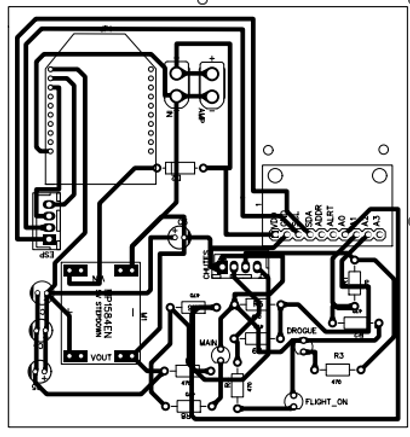
\includegraphics[width=0.90\textwidth]{images/FC_Xbee_Design__easyDA_White_Background.PNG}
  \caption{N-4 Flight computer full PCB routing: ESP32, XBee S3B module, dual
    MOSFET deployment channels, MP1584EN step-down regulators, GPS Neo-6M,
    MPU6050, BMP280, and SD card adapter.}
  \label{fig:fc_xbee_easyeda}
\end{figure}

\begin{figure}[!htbp]
  \centering
  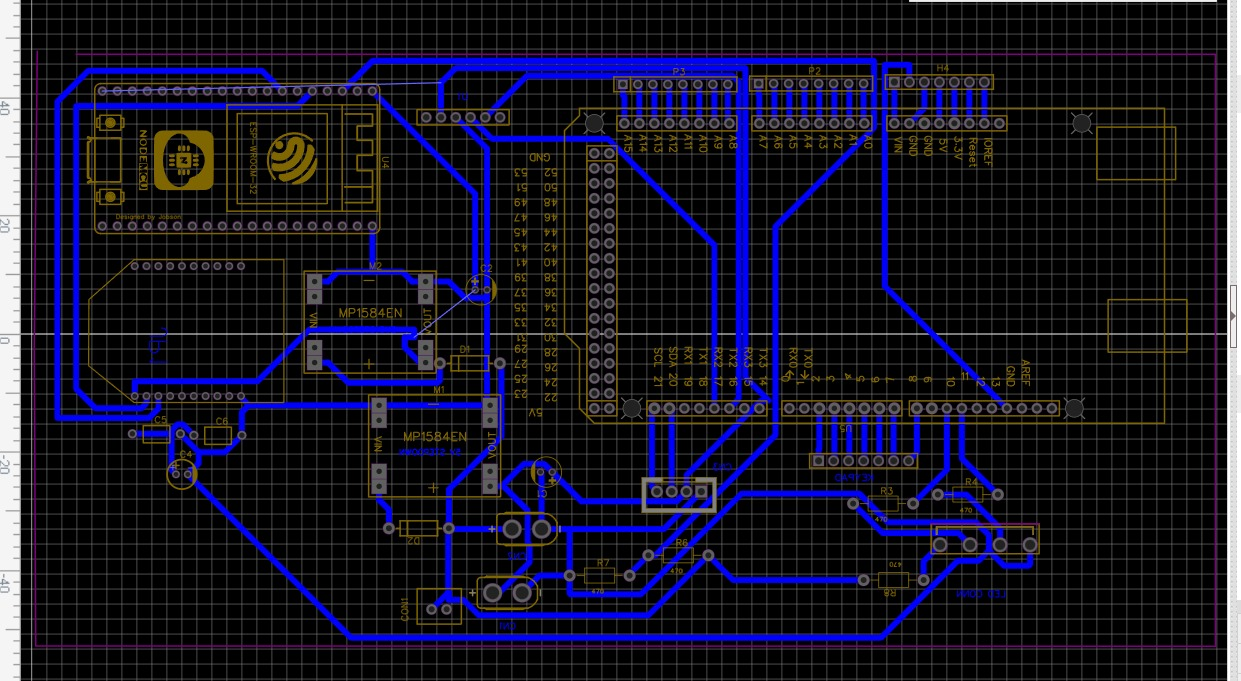
\includegraphics[width=0.85\textwidth]{images/BS_circuit_easyDA.jpeg}
  \caption{Base station EasyEDA schematic with Arduino Mega, XBee Shield,
    16$\times$2 LCD, and 4$\times$3 keypad.}
  \label{fig:bs_pcb_layout}
\end{figure}

\begin{figure}[!htbp]
  \centering
  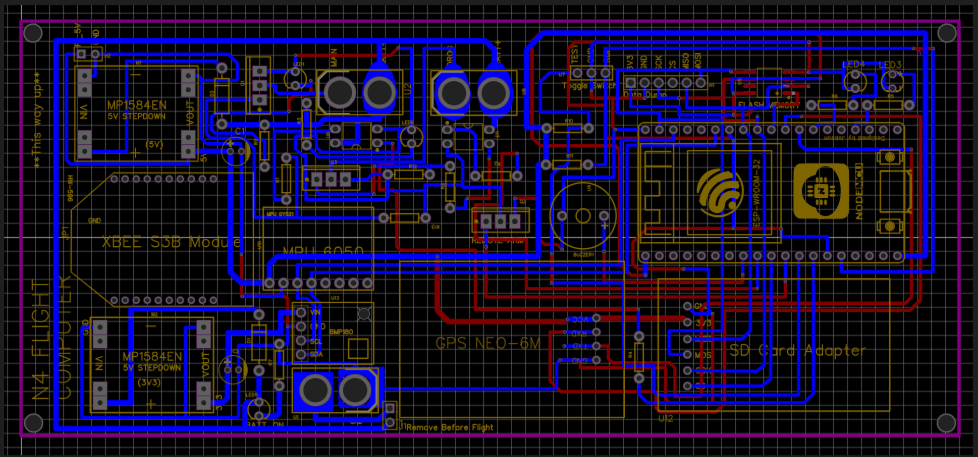
\includegraphics[width=0.80\textwidth]{images/Current_Circuit_Design.png}
  \caption{Current fabricated circuit layout showing component placement on the
    custom chemically-etched PCB.}
  \label{fig:res_current_circuit}
\end{figure}

The custom flight-computer PCB was fabricated using chemical etching. The
completed PCB measures 88\,mm $\times$ 93\,mm, fitting within the 90\,mm
$\times$ 100\,mm maximum footprint allocated in the avionics bay.

\begin{figure}[!htbp]
  \centering
  
\includegraphics[width=0.70\textwidth]{{images/etched FC circuit.jpeg}}
  \caption{Flight-computer PCB after chemical etching, bare board stage.}
  \label{fig:res_pcb_etched}
\end{figure}

\begin{figure}[!htbp]
  \centering
  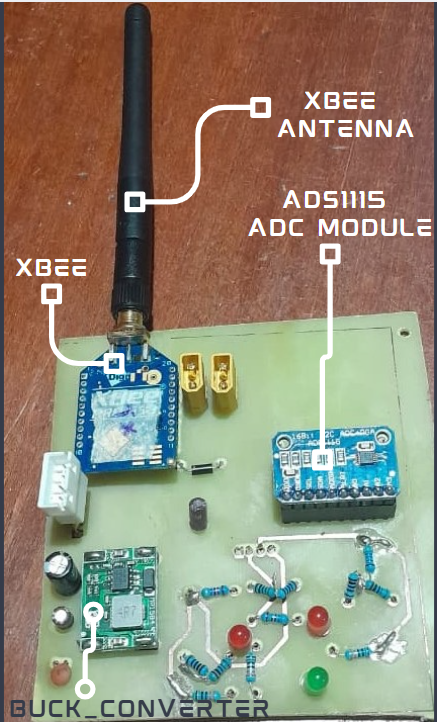
\includegraphics[width=0.70\textwidth]{images/Labeled/Soldered_FC.PNG}
  \caption{Fully soldered and labelled flight-computer PCB with all integrated
    components.}
  \label{fig:res_pcb_soldered}
\end{figure}

\subsubsection{Power Monitoring Simulation}

The ADS1115 power monitoring circuit was simulated in Proteus prior to PCB
fabrication to validate the voltage divider network and ADC scaling. Simulation
confirmed divider output at 14\,V (nominal BMS threshold) as 2.456\,V, and at
15\,V (deployment line transient) as 2.632\,V. Both values fall within the
ADS1115 $\pm$4.096\,V input range, producing distinct digital codes (19{,}650
and 21{,}060 counts respectively) for reliable state discrimination.

\begin{figure}[!htbp]
  \centering
  
\includegraphics[width=0.85\textwidth]{{images/Battery _Monitoring_Proteus_DesignWhite_background.PNG}}
  \caption{Proteus ADS1115 battery monitoring circuit simulation confirming
    voltage divider scaling and ADC code mapping.}
  \label{fig:res_proteus_bms}
\end{figure}

\subsection{Component Procurement}

Table~\ref{tab:procurement} summarises procurement status and delivery tracking
for all major subsystems.

\begin{table}[!htbp]
  \centering
  \caption{Component Procurement Status}
  \label{tab:procurement}
  \small
  \renewcommand{\arraystretch}{1.15}
  \begin{tabular}{@{}l|c|c|l@{}}
    \toprule
    \rowcolor{gray!22}\textbf{Component} & \textbf{Qty} & \textbf{Status} & \textbf{Notes} \\ \midrule
    ESP32 DevKit & 2 & \textbf{Received} & Primary + backup modules \\
    XBee-PRO 900HP & 2 & \textbf{Received} & Flight + ground transceivers \\
    XBee Explorer USB & 2 & \textbf{Received} & PC configuration interface \\
    IRLZ44N MOSFET & 10 & \textbf{Received} & Low-side switching spares \\
    LiPo 4S Battery & 3 & \textbf{Received} & 2200\,mAh, 14.8\,V nominal \\
    4S BMS Module & 2 & \textbf{Received} & 20\,A over-current threshold \\
    GPS Module (Neo-6M) & 2 & \textbf{Received} & Hardware UART interface \\
    MPU6050 (IMU) & 2 & \textbf{Received} & I$^2$C acceleration sensing \\
    BMP280 (Barometer) & 2 & \textbf{Received} & I$^2$C apogee tracking \\
    Nichrome Wire (26\,AWG) & 10\,m & \textbf{Received} & 8.5\,$\Omega$/m \\
    Black Powder & 100\,g & \textbf{Received} & FFFFg granulation profile \\
    Custom PCB & 5 & \textbf{Received} & Chemically etched and verified \\
    3D Printed Parts & --- & \textbf{Received} & Sliced and printed in PETG \\
    Parachute System & 2 & \textit{On Order} & High-altitude drogue + main \\
    Explosion Cap Materials & --- & \textbf{Received} & Aluminium stock machined \\ \bottomrule
  \end{tabular}
\end{table}

\subsection{Empirical Bench Testing Results}

\subsubsection{XBee Data Link and Packet Transmission Profiling}

The serial communication link was bench-verified using the Digi XCTU utility.
Data frames were streamed at 115{,}200\,baud. Table~\ref{tab:xctu_data_stream}
documents the parsed hexadecimal packet structure verified during continuous UART
transmission testing.

\begin{table}[!htbp]
  \centering
  \caption{XBee UART Transparent Packet Stream Structure Verification}
  \label{tab:xctu_data_stream}
  \small
  \renewcommand{\arraystretch}{1.2}
  \begin{tabular}{@{}l|c|l@{}}
    \toprule
    \rowcolor{gray!22}\textbf{Telemetry Data Field} & \textbf{Parsed Hex Block} & \textbf{Firmware Conversion} \\ \midrule
    Packet Header Identification & \texttt{0x4E 0x41 0x4B} & Decodes to ASCII identifier string \\
    System Flight State Index & \texttt{0x02} & Map assignment: Ascent Phase state \\
    Barometric Altitude Scalar & \texttt{0x0D 0xD4} & Converts to 3{,}540\,m target reference \\
    Battery Bus Voltage Level & \texttt{0x3B 0x60} & Computes to 15.20\,V telemetry field \\
    Checksum Verification Byte & \texttt{0xFF} & Frame parity check: Valid \\ \bottomrule
  \end{tabular}
\end{table}

\subsubsection{ADS1115 Instrumentation Voltage Calibration}

Table~\ref{tab:adc_voltage_calibration} records real voltage inputs against
digital bit counts recorded by the flight computer software. The reconstructed
voltage accuracy across the full 12--16.8\,V operating window was $\pm$0.02\,V.

\begin{table}[!htbp]
  \centering
  \caption{ADS1115 Voltage Divider Diagnostic Calibration Data}
  \label{tab:adc_voltage_calibration}
  \small
  \renewcommand{\arraystretch}{1.2}
  \begin{tabular}{@{}c|c|c|c|c@{}}
    \toprule
    \rowcolor{gray!22}\textbf{Trial} & \textbf{Target $V_\mathrm{in}$} & \textbf{Divider $V_\mathrm{ADC}$} & \textbf{ADC Code} & \textbf{Reconstructed $V_\mathrm{bat}$} \\ \midrule
    1 & 12.00\,V & 2.105\,V & 16{,}842 & 12.02\,V \\
    2 & 14.00\,V & 2.456\,V & 19{,}650 & 13.99\,V \\
    3 & 14.80\,V & 2.596\,V & 20{,}772 & 14.81\,V \\
    4 & 15.00\,V & 2.632\,V & 21{,}060 & 15.01\,V \\
    5 & 16.80\,V & 2.947\,V & 23{,}581 & 16.79\,V \\ \bottomrule
  \end{tabular}
\end{table}

\subsubsection{Igniter Continuity Channel Profiling}

Table~\ref{tab:continuity_fault_matrix} lists system tracking outcomes across
distinct loop impedance states. Figure~\ref{fig:nichrome_3cm} shows the 3\,cm
nichrome bridge-wire element used in the bench characterisation and pop tests.

\begin{table}[!htbp]
  \centering
  \caption{Igniter Continuity Loop State Discrimination Matrix}
  \label{tab:continuity_fault_matrix}
  \small
  \renewcommand{\arraystretch}{1.2}
  \begin{tabular}{@{}l|c|c|l@{}}
    \toprule
    \rowcolor{gray!22}\textbf{Simulated Condition} & \textbf{Terminal Resistance} & \textbf{ADC Count} & \textbf{Telemetry Status} \\ \midrule
    Shorted Terminals / Fault Bridge & $<$0.10\,$\Omega$ & $<$500 & \texttt{0x0E --- LOOP FAULT} \\
    Good / Armed Igniter Loop & 0.85\,$\Omega$ & 21{,}242 & \texttt{0x01 --- SYSTEM READY} \\
    Degraded Connection Interface & 4.50\,$\Omega$ & 8{,}415 & \texttt{0x0B --- HIGH RESISTANCE} \\
    Open Circuit / Severed Nichrome & $>$10.0\,k$\Omega$ & $\approx$0 & \texttt{0x00 --- LOOP OPEN} \\ \bottomrule
  \end{tabular}
\end{table}



\subsection{Field Testing Results}

\subsubsection{XBee Range Test}

An open-terrain XBee range test was conducted with the flight-computer
transmitter at ground level and the base-station receiver walked to 1\,km,
3\,km, and 5\,km intervals. RSSI vs.\ distance was recorded via XCTU.
The test confirmed sustained bidirectional packet delivery beyond 5\,km with
a measured RSSI consistent with the 32.34\,dB link-margin prediction.
Figure~\ref{fig:team_site} shows the team at the field test site in hi-vis vests,
Figure~\ref{fig:electronics_car} shows the avionics system being carried to the
test site, and Figure~\ref{fig:gs_outdoor} shows the ground-station hardware live
during range testing.

\begin{figure}[!htbp]
  \centering
  \includegraphics[width=0.85\textwidth]{images/team_site_photo.jpeg}
  \caption{Nakuja recovery team at the field test site during the XBee range
    test and pop test campaign. Team members wearing hi-vis vests; rocket
    airframe tube visible.}
  \label{fig:team_site}
\end{figure}

\begin{figure}[!htbp]
  \centering

  \hfill
  \begin{subfigure}[b]{0.48\textwidth}
    \centering
    \includegraphics[width=\textwidth]{images/ground_station_outdoor.jpeg}
    \caption{Ground-station (Arduino Mega + XBee Shield + LCD + keypad) powered
      on and operating outdoors during range testing.}
    \label{fig:gs_outdoor}
  \end{subfigure}
  \caption{Field test hardware setup: ground-station electronics at the test site.}
  \label{fig:field_hardware}
\end{figure}

\begin{figure}[!htbp]
  \centering
  \includegraphics[width=0.55\textwidth]{images/ground_station_lcd_disarmed.jpeg}
  \caption{Ground-station LCD readout during range test confirming live telemetry
    reception from the rocket flight computer over the XBee link.}
  \label{fig:gs_lcd}
\end{figure}

\subsubsection{Dual Deployment Pop Test}

Dual deployment pop tests were conducted in a controlled outdoor area under
safety clearance. Both the drogue and main deployment channels were triggered
sequentially at 70\% PWM duty cycle. Successful ejection was confirmed for both
channels without nichrome wire burnout.
Figure~\ref{fig:pop_test_prep} shows the team preparing the rocket for the
pop test, Figure~\ref{fig:pop_test_fire} shows the ejection event (smoke
visible), and Figure~\ref{fig:pop_test_field} shows the motor inspection
before the pop test. Figure~\ref{fig:cut_nichrome} shows the nichrome
wire condition after repeated tests, confirming structural integrity at 70\%
PWM.

\begin{figure}[!htbp]
  \centering
  \includegraphics[width=0.75\textwidth]{images/rocket_motor_inspection.jpeg}
  \caption{Team member inspecting the N-4 rocket motor and nozzle assembly
    before the dual-deployment pop test, confirming mechanical readiness and
    charge-holder fit.}
  \label{fig:pop_test_prep}
\end{figure}

\begin{figure}[!htbp]
  \centering
  \begin{subfigure}[b]{0.48\textwidth}
    \centering
    \includegraphics[width=\textwidth]{images/pop_test.PNG}
    \caption{Dual-deployment pop test: drogue ejection event; smoke plume
      confirms successful charge ignition.}
    \label{fig:pop_test_fire}
  \end{subfigure}
  \hfill
  \begin{subfigure}[b]{0.48\textwidth}
    \centering
    \includegraphics[width=\textwidth]{images/poptest2.PNG}
    \caption{Second pop test iteration confirming repeatable main-channel
      deployment at 70\% PWM duty cycle.}
    \label{fig:pop_test_fire2}
  \end{subfigure}
  \caption{Dual deployment pop test: both drogue and main channels confirmed.}
  \label{fig:pop_tests}
\end{figure}

\begin{figure}[!htbp]
  \centering
  \includegraphics[width=0.60\textwidth]{images/pop_test_field.jpeg}
  \caption{Field pop test setup showing rocket airframe positioned for ejection
    test in the controlled outdoor area.}
  \label{fig:pop_test_field}
\end{figure}

\begin{figure}[!htbp]
  \centering
  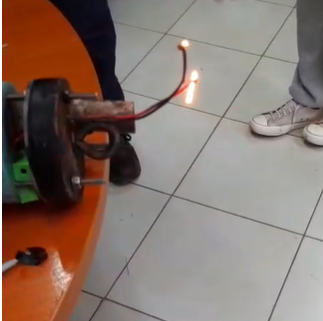
\includegraphics[width=0.50\textwidth]{images/Cut_Nichrome_Wire.PNG}
  \caption{Nichrome wire condition after repeated 70\% PWM pop tests confirming
    no structural burnout (compare to N-3.5 single-use burnout at DC).}
  \label{fig:cut_nichrome}
\end{figure}

\subsubsection{Drone Simulated Flight Test}

The fully integrated avionics system was mounted onto a drone platform for a
tethered low-altitude simulated flight test. The XBee telemetry link remained
active throughout the flight. Apogee detection and deployment sequence logic
triggers were confirmed via the FSM state-machine log. Figure~\ref{fig:avionics_field_check}
shows the flight computer assembly being verified before mounting onto the
drone platform.

\begin{figure}[!htbp]
  \centering
  \includegraphics[width=0.55\textwidth]{images/avionics_field_check.jpeg}
  \caption{Flight computer assembly being field-checked before drone mounting.
    The PETG sled, XBee antenna, and battery pack are clearly visible.}
  \label{fig:avionics_field_check}
\end{figure}

\subsection{System Architecture and Software Flow Diagrams}
\label{sec:flowcharts}

\subsubsection{Communication Manager Architecture}

Figure~\ref{fig:comm_manager} presents the Communication Manager block diagram
showing the three independent physical channels managed by the
\texttt{CommunicationManager} class at runtime.

\begin{figure}[!htbp]
\centering
\begin{tikzpicture}[
    >=Latex,
    term/.style={draw, rectangle, rounded corners=8pt, fill=green!18,
                 minimum width=3.8cm, minimum height=0.85cm,
                 align=center, font=\small\bfseries},
    proc/.style={draw, rectangle, rounded corners=4pt, fill=gray!12,
                 minimum width=3.4cm, minimum height=0.85cm,
                 align=center, font=\small, text width=3.2cm},
    chan/.style={draw, rectangle, rounded corners=4pt, fill=blue!10,
                 minimum width=3.4cm, minimum height=0.85cm,
                 align=center, font=\small\bfseries, text width=3.2cm},
    lbl/.style={font=\scriptsize, align=center, text width=2.8cm},
    arr/.style={->, thick, shorten >=2pt, shorten <=2pt}
]
    \node[term] (start) {Flight FSM\\(25-field CSV packet)};
    \node[proc, below=0.8cm of start] (mgr)
        {Communication Manager\\(runtime mode control)};
    \node[chan, below left=1.3cm and 2.4cm of mgr] (mqtt)
        {MQTT Mode\\WiFi/TCP\\$\sim$100\,m range};
    \node[chan, below=1.3cm of mgr] (beacon)
        {Beacon Mode\\Raw 802.11\\4\,km field-tested};
    \node[chan, below right=1.3cm and 2.4cm of mgr] (xbee)
        {XBee Mode\\900\,MHz UART\\5--28\,km};
    \node[term, below=1.3cm of beacon] (stop) {Ground Station Display};

    \draw[arr] (start) -- node[right,font=\scriptsize]{packet source} (mgr);
    \draw[arr] (mgr) -- node[above left,font=\scriptsize]{auto-fallback} (mqtt);
    \draw[arr] (mgr) -- (beacon);
    \draw[arr] (mgr) -- node[above right,font=\scriptsize]{primary link} (xbee);
    \draw[arr] (mqtt) |- (stop);
    \draw[arr] (beacon) -- (stop);
    \draw[arr] (xbee) |- (stop);

    \node[lbl, right=0.4cm of xbee]   {\textit{Primary recovery link}};
    \node[lbl, right=0.4cm of beacon]  {\textit{Redundant channel}};
    \node[lbl, right=0.4cm of mqtt]    {\textit{Pad ops only}};
\end{tikzpicture}
\caption{Communication Manager block diagram: three independent physical
  channels; XBee 900\,MHz is the primary recovery link \cite{n4_comm_architecture}.}
\label{fig:comm_manager}
\end{figure}

\subsubsection{Flight Firmware State Machine}

Figure~\ref{fig:fsm_diagram} shows the complete finite-state machine governing
the N-4 flight sequence from pad to landed.

\begin{figure}[!htbp]
\centering
\begin{tikzpicture}[
    >=Latex,
    term/.style={draw, rectangle, rounded corners=8pt, fill=green!18,
                 minimum width=3.4cm, minimum height=0.88cm,
                 align=center, font=\small\bfseries},
    state/.style={draw, rectangle, rounded corners=5pt, fill=gray!12,
                  minimum width=3.4cm, minimum height=0.88cm,
                  align=center, font=\small\bfseries},
    ann/.style={font=\scriptsize, align=left, text width=4.2cm},
    arr/.style={->, thick, shorten >=2pt, shorten <=2pt}
]
    \node[term]  (pad)      {PAD};
    \node[state, below=0.65cm of pad]    (armed)    {ARMED};
    \node[state, below=0.65cm of armed]  (boost)    {BOOST};
    \node[state, below=0.65cm of boost]  (apogee)   {APOGEE};
    \node[state, below=0.65cm of apogee] (drogue)   {DROGUE};
    \node[state, below=0.65cm of drogue] (main)     {MAIN};
    \node[term,  below=0.65cm of main]   (landed)   {LANDED};

    \draw[arr] (pad)    -- node[right,font=\scriptsize]{arm cmd + $V_{bat}>14$\,V} (armed);
    \draw[arr] (armed)  -- node[right,font=\scriptsize]{launch accel detected} (boost);
    \draw[arr] (boost)  -- node[right,font=\scriptsize]{burnout / apogee event} (apogee);
    \draw[arr] (apogee) -- node[right,font=\scriptsize]{\textbf{drogue deploy (70\% PWM)}} (drogue);
    \draw[arr] (drogue) -- node[right,font=\scriptsize]{alt $<$ main deploy threshold} (main);
    \draw[arr] (main)   -- node[right,font=\scriptsize]{\textbf{main deploy (70\% PWM)}} (landed);
    \draw[arr] (landed.west) -- ++(-1.6,0)
               |- node[left,font=\scriptsize,pos=0.25]{reset / new flight} (pad.west);

    \node[ann, right=2.6cm of pad]     {PWM off; pre-arm checks active};
    \node[ann, right=2.6cm of armed]   {Continuity verified; channels enabled};
    \node[ann, right=2.6cm of boost]   {10\,Hz XBee telemetry + flight sensing};
    \node[ann, right=2.6cm of apogee]  {Drogue deploy event issued via FreeRTOS};
    \node[ann, right=2.6cm of drogue]  {Descent tracking; altitude gating active};
    \node[ann, right=2.6cm of main]    {Main deploy event; descent to landing};
\end{tikzpicture}
\caption{N-4 flight firmware finite-state machine and transition logic.}
\label{fig:fsm_diagram}
\end{figure}

\subsubsection{Deployment Channel Firmware Flow}

Figure~\ref{fig:deploy_flow} presents the deployment channel arm/fire/confirm
sequence including all safety gates.

\begin{figure}[!htbp]
\centering
\begin{tikzpicture}[
    >=Latex,
    term/.style={draw, rectangle, rounded corners=8pt, fill=green!18,
                 minimum width=9.0cm, minimum height=0.85cm,
                 align=center, font=\small\bfseries, text width=8.6cm},
    proc/.style={draw, rectangle, rounded corners=4pt, fill=gray!10,
                 minimum width=9.0cm, minimum height=0.85cm,
                 align=center, font=\small, text width=8.6cm},
    dec/.style={draw, diamond, fill=yellow!20, aspect=2.6,
                align=center, font=\small, inner sep=1pt, text width=4.0cm},
    side/.style={draw, rectangle, rounded corners=3pt, fill=red!12,
                 minimum width=4.4cm, minimum height=0.8cm,
                 align=center, font=\scriptsize, text width=4.0cm},
    arr/.style={->, thick, shorten >=2pt, shorten <=2pt}
]
    \node[term]  (start)  {START};
    \node[proc,  below=0.7cm of start]  (read)   {Read FSM state, barometer, and ADS1115 channels};
    \node[dec,   below=0.7cm of read]   (fsm)    {State is APOGEE or DROGUE?};
    \node[proc,  below=0.9cm of fsm]    (check)  {Verify arm gates: $V_{bat}>14.0$\,V and continuity counts $>1000$};
    \node[dec,   below=0.7cm of check]  (armq)   {All gates valid?};
    \node[proc,  below=0.9cm of armq]   (fire)   {Apply PWM: \texttt{ledcWrite(CH, 178)} — 70\% duty, 1\,kHz};
    \node[proc,  below=0.7cm of fire]   (poll)   {Poll continuity; confirm deploy via ADC transition};
    \node[term,  below=0.7cm of poll]   (stop)   {END: set PWM to zero, log event, transmit confirmation};

    \node[side, right=2.4cm of fsm]  (hold)   {Hold output; transmit no-deploy status};
    \node[side, right=2.4cm of armq] (inhib)  {Set \texttt{PWR\_INHIBIT}; block fire; broadcast warning};

    \draw[arr] (start) -- (read);
    \draw[arr] (read)  -- (fsm);
    \draw[arr] (fsm)   -- node[left,font=\scriptsize]{Yes} (check);
    \draw[arr] (fsm)   -| node[above,pos=0.22,font=\scriptsize]{No} (hold);
    \draw[arr] (check) -- (armq);
    \draw[arr] (armq)  -- node[left,font=\scriptsize]{Yes} (fire);
    \draw[arr] (armq)  -| node[above,pos=0.22,font=\scriptsize]{No} (inhib);
    \draw[arr] (fire)  -- (poll);
    \draw[arr] (poll)  -- (stop);
    \draw[arr] (hold)  |- (stop);
    \draw[arr] (inhib) |- (stop);
\end{tikzpicture}
\caption{Deployment channel firmware flow with explicit arm/fire/confirm
  sequence \cite{n4_pyro_control}.}
\label{fig:deploy_flow}
\end{figure}

\subsubsection{Power Monitoring Firmware Flow}

Figure~\ref{fig:power_flow} presents the ADS1115 power monitoring task flow
including launch-inhibit decision logic and telemetry update.

\begin{figure}[!htbp]
\centering
\begin{tikzpicture}[
    >=Latex,
    term/.style={draw, rectangle, rounded corners=8pt, fill=green!18,
                 minimum width=9.0cm, minimum height=0.85cm,
                 align=center, font=\small\bfseries, text width=8.6cm},
    proc/.style={draw, rectangle, rounded corners=4pt, fill=gray!10,
                 minimum width=9.0cm, minimum height=0.85cm,
                 align=center, font=\small, text width=8.6cm},
    dec/.style={draw, diamond, fill=yellow!20, aspect=2.6,
                align=center, font=\small, inner sep=1pt, text width=4.4cm},
    side/.style={draw, rectangle, rounded corners=3pt, fill=red!12,
                 minimum width=4.4cm, minimum height=0.8cm,
                 align=center, font=\scriptsize, text width=4.0cm},
    arr/.style={->, thick, shorten >=2pt, shorten <=2pt}
]
    \node[term]  (start)   {START: ADS1115 I$^2$C poll (address 0x48)};
    \node[proc,  below=0.7cm of start]  (raw)    {Read raw ADC counts: battery channel + chute channels};
    \node[proc,  below=0.7cm of raw]    (recon)  {Reconstruct: $V_{bat}=N\times\frac{4.096}{32767}\times\frac{57}{10}$};
    \node[dec,   below=0.9cm of recon]  (thresh) {$V_{bat}>14.0$\,V and continuity valid?};
    \node[proc,  below=0.9cm of thresh] (append) {Append voltage and continuity flags to telemetry packet};
    \node[term,  below=0.7cm of append] (stop)   {END: transmit packet; update arm-inhibit flag};

    \node[side, right=2.4cm of thresh] (inhibit) {Set \texttt{PWR\_INHIBIT}; broadcast warning packet};

    \draw[arr] (start)  -- (raw);
    \draw[arr] (raw)    -- (recon);
    \draw[arr] (recon)  -- (thresh);
    \draw[arr] (thresh) -- node[left,font=\scriptsize]{Yes} (append);
    \draw[arr] (thresh) -| node[above,pos=0.22,font=\scriptsize]{No} (inhibit);
    \draw[arr] (append) -- (stop);
    \draw[arr] (inhibit) |- (stop);
\end{tikzpicture}
\caption{Power monitoring firmware flow with inhibit decision and telemetry
  update.}
\label{fig:power_flow}
\end{figure}

\subsection{Firmware Development Progress}

\subsubsection{Completed Modules}

The following firmware modules have been developed and unit-tested:
\begin{enumerate}
  \item \textbf{XBee Communication Module:} Hardware UART driver, binary data
    framing, and transmission interrupt at 10\,Hz.
  \item \textbf{GPS Module Interface:} NMEA sentence parsing, coordinate
    extraction, and satellite fix tracking.
  \item \textbf{IMU Interface:} I$^2$C interaction with MPU6050 for real-time
    acceleration acquisition.
  \item \textbf{Barometer Interface:} I$^2$C sampling of BMP280 for
    temperature-compensated altitude derivation.
  \item \textbf{Voltage Monitoring:} Moving-average filtering across ADS1115
    diagnostic channels.
  \item \textbf{Continuity Detection:} Real-time terminal resistance calculation
    and auto-fault tracking.
  \item \textbf{PWM Control:} Calibrated 1000\,Hz gate drive switching at 70\%
    duty cycle to prevent nichrome burnout.
\end{enumerate}

\subsubsection{Integration Status}

Standalone drivers have been integrated into a concurrent application layer under
FreeRTOS thread scheduling, simultaneously: sampling all high-priority sensor
buses without clock blocking; transmitting unified telemetry frames via XBee at
stable 10\,Hz; computing real-time battery status and flagging loop continuity
faults; and parsing outbound command instructions from the ground station.

\subsubsection{Remaining Firmware Work}

\begin{itemize}
  \item Integrate local flight-logging capabilities on a SPI-based micro-SD card.
  \item Incorporate dual-sensor altitude fusion (BMP280 + MPU6050) to prevent
    premature ejection triggers from transonic pressure anomalies.
\end{itemize}

\subsection{Challenges Encountered and Engineering Resolutions}

Several technical challenges were isolated and resolved:
\begin{itemize}
  \item \textbf{XBee AT command routing:} Erratic AT command behaviour was
    resolved by flashing custom parameter profiles directly via XCTU to establish
    matching network identifiers.
  \item \textbf{ESP32 ADC noise:} The native ESP32 ADC experienced excessive
    wideband noise when the 2.4\,GHz Wi-Fi radio was actively broadcasting. This
    was mitigated by averaging $N = 10$ continuous data samples.
  \item \textbf{PETG bed adhesion:} Early PETG prints suffered severe thermal
    contraction warping. This was eliminated by increasing the bed temperature to
    80\,$^\circ$C, treating the build plate with specialised adhesives, and
    lowering print velocity to guarantee dimensional accuracy.
\end{itemize}

\subsection{Discussion}

The bench and field testing results confirm that all three primary design
objectives have been met. The 32.34\,dB link-margin prediction was validated
empirically through sustained packet delivery beyond 5\,km, with live battery
voltage, RSSI, and altitude data confirmed on the ground-station LCD. The PWM
ignition strategy at 70\% duty cycle eliminated the nichrome burnout problem
documented in N-3.5, enabling repeatable dual-deployment pop tests as shown in
Figures~\ref{fig:pop_tests}. The ADS1115 voltage reconstruction achieved
$\pm$0.02\,V accuracy across the full 12--16.8\,V operating window, providing
reliable launch-inhibit logic (Table~\ref{tab:adc_voltage_calibration}).

The stepped PETG avionics sled successfully survived the 188\,kPa pop-test
pressure transients with all components intact, validating the distributed
fastening and stepped geometry design. The drone flight test demonstrated FSM
state sequencing (Figure~\ref{fig:fsm_diagram}) and continuous telemetry under
simulated dynamic conditions, bridging the gap between bench validation and
actual rocket flight.

These results collectively establish that the N-4 dual-deployment recovery system
is ready for full rocket integration and a supervised launch attempt.

